%!TEX program = xelatex

\documentclass[varwidth,convert]{BHCexam1_simple}
\usepackage{gensymb}
\usepackage{mathrsfs}
\usepackage{tikz,pgfplots,float} %绘图
\usepackage{tkz-euclide}
\usepackage{graphicx}
\usepackage{wrapfig}
\usepackage[english]{babel}
\usepackage{caption}
\usepackage{CJK}
\usepackage{enumitem}
\usetikzlibrary{calc,quotes,angles,babel,intersections,arrows,automata,positioning}

\pgfplotsset{compat=1.15}
\tikzset{ 
  right angle quadrant/.code={ 
   \pgfmathsetmacro\quadranta{{1,1,-1,-1}[#1-1]} % Arrays for selecting quadrant 
   \pgfmathsetmacro\quadrantb{{1,-1,-1,1}[#1-1]}}, 
  right angle quadrant=1, % Make sure it is set, even if not called explicitly 
  right angle length/.code={\def\rightanglelength{#1}}, % Length of symbol 
  right angle length=2ex, % Make sure it is set... 
  right angle symbol/.style n args={3}{ 
   insert path={ 
   let \p0 = ( $(#1)!(#3)!(#2)$ ) in % Intersection 
    let \p1 = ( $(\p0)!\quadranta*\rightanglelength!(#3)$ ), % Point on base line 
    \p2 = ( $(\p0)!\quadrantb*\rightanglelength!(#2)$ ) in % Point on perpendicular line 
    let \p3 = ( $(\p1)+(\p2)-(\p0)$ ) in % Corner point of symbol 
   (\p1) -- (\p3) -- (\p2) 
   } 
  } 
}

\setlength{\textwidth}{20cm}

\begin{document}

%%% -------- Anchor Start -------- %%%

如图,在$\triangle ABC$中,$\angle ACB=90\degree$,$\angle A=30 \degree,~D$是边$AC$上不与点$A$、$C$重合的任意一点,
$DE\bot AB$,垂足为点$E$,$M$是$BD$的中点.
% \stk{}

\begin{enumerate}[label={(\arabic*)}]
\item 求证:$CM=EM$~;
\item 如果~$BC=\sqrt{3}$,设~$AD=x,~CM=y$,求$y$与$x$的函数解析式,并写出定义域;
\item 当点$D$在线段$AC$上移动时,$\angle MCE$~的大小是否发生变化?若不变,求出~$\angle MCE$~的大小;如果发生变化,说明如何变化.
\end{enumerate}
% \twoch{a}{b}{c}{d}
\hfill
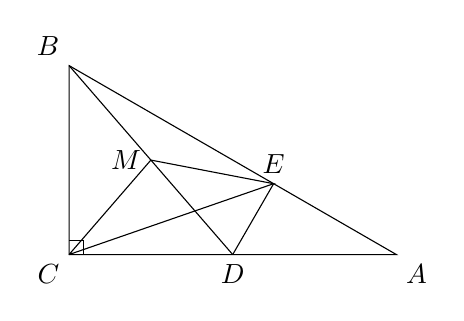
\begin{tikzpicture}[scale=0.6]
%\draw [help lines] (0,0) grid (7,4);
\coordinate[label=below left:$C$] (C) at (0,0);
\coordinate[label=above left:$B$] (B) at (0,4);
\coordinate[label=below right:$A$] (A) at ({4*sqrt(3)},0);
\draw [right angle symbol={B}{C}{A}]; 
\draw (A) -- (B) -- (C) -- cycle;
\coordinate[label=below:$D$] (D) at($(C)!0.5!(A)$);
\draw (B) -- (D);
\draw ( $(A)!(D)!(B)$ ) coordinate[label=above:$E$] (E) -- (D); 
\coordinate[label=left:$M$] (M) at($(B)!0.5!(D)$);
\draw (C) -- (M) -- (E) -- (C);
% \draw[blue,->] (C) -- ($(A)!(C)!(B)$);
\end{tikzpicture}

%%% -------- Anchor Start -------- %%%

\end{document}